\chapter{Énergie, courbure et rayonnement}

\lectureoverview{Le modèle newtonien devient beaucoup plus instructif dès que l’on lève deux restrictions. Premièrement, l’énergie totale d’une galaxie comobile n’a pas besoin d’être exactement nulle : la laisser arbitraire fait apparaître le terme \(a^{-2}\), que la relativité générale réinterprétera comme une courbure spatiale. Deuxièmement, la source cosmique n’a pas besoin d’être constituée de matière sans pression. La longueur d’onde des photons s’étire avec le facteur d’échelle, de sorte que le rayonnement se dilue comme \(a^{-4}\) et entraîne la loi \(a(t)\propto t^{1/2}\). Un univers contenant à la fois matière et rayonnement est donc dominé par le rayonnement aux petites valeurs de \(a\), puis par la matière aux valeurs plus grandes de \(a\). Nous distinguerons au fil de l’exposé le mouvement newtonien local de la géométrie relativiste globale et repérerons les questions auxquelles seule la relativité générale permet de répondre.}

\section{Ce que Newton peut décrire}

Avant d’étendre le modèle, demandons-nous pourquoi le calcul newtonien précédent a fonctionné. L’univers physique est décrit par la relativité générale, et sa géométrie spatiale n’est pas nécessairement euclidienne à l’échelle globale. Pourtant, tout espace courbe régulier est approximativement plat dans un voisinage suffisamment petit. Une petite portion de la surface terrestre paraît plane ; de même, une région de l’univers beaucoup plus petite que son rayon de courbure peut être traitée comme plate.

``Petit'' signifie ici petit par rapport à l’échelle de courbure. La région peut néanmoins s’étendre sur des milliards d’années-lumière. Dans celle-ci, on peut décrire les galaxies voisines par la mécanique newtonienne lorsque leurs vitesses particulières relatives sont non relativistes et que le champ gravitationnel est faible. Le calcul newtonien ne rivalise donc pas avec la théorie d’Einstein : il en constitue la limite locale à faible vitesse.

Une mise en garde s’impose d’emblée. Le rayonnement ne se déplace pas lentement. Les photons, ainsi que les neutrinos tant qu’ils sont relativistes, ne peuvent pas être traités comme un gaz de particules newtoniennes ordinaires. Le raisonnement newtonien continuera à organiser l’équation d’expansion, mais il faudra remplacer, dans son membre de droite, la densité de masse au repos par la densité d’énergie. C’est là que l’approximation commence à révéler ses propres limites.

\section{Rappel sur le facteur d’échelle}

Considérons une distribution homogène de galaxies et associons des coordonnées à une grille qui se déplace avec le flot cosmique moyen. Une galaxie de coordonnée comobile fixe \(x\) se trouve à la distance physique
\begin{equation}
D(t)=a(t)x
\label{eq:c02-distance}
\end{equation}
de l’origine choisie. Le facteur d’échelle \(a(t)\) convertit la séparation en coordonnées en séparation physique.

La valeur absolue de \(a\) est conventionnelle. Si l’on redéfinit toutes les coordonnées comobiles en les multipliant par une constante, les mêmes distances physiques peuvent être représentées en multipliant \(a\) par la constante inverse. Ainsi, ni \(a\) ni la masse attribuée à une cellule de coordonnées ne sont invariantes séparément. Les rapports de facteurs d’échelle et le taux d’expansion fractionnaire sont invariants :
\begin{equation}
\frac{a(t_2)}{a(t_1)},
\qquad
H(t)\equiv\frac{\dot a}{a}.
\label{eq:c02-hubble}
\end{equation}
En effet, si \(a'=\alpha a\) pour une constante fixe \(\alpha\), alors \(\dot a'/a'=\dot a/a\).

Soit \(\nu_m\) la masse contenue dans une unité de volume en coordonnées comobiles. Sa valeur numérique change si l’on redéfinit la grille, mais elle reste constante dans le temps lorsque la matière ordinaire se conserve. Un cube comobile d’unité de côté a un volume physique \(a^3\) ; la densité de matière vaut donc
\begin{equation}
\boxed{\rho_m(a)=\frac{\nu_m}{a^3}.}
\label{eq:c02-matter-density}
\end{equation}
Cette dilution en \(a^{-3}\) est simplement due à l’augmentation du volume : l’énergie au repos contenue dans la boîte comobile reste constante tandis que son volume augmente.

Les galaxies réelles ne sont pas rigidement fixées à la grille. Elles gravitent dans des groupes, tombent dans des amas et ont de petites vitesses par rapport au flot moyen. Le facteur d’échelle décrit le mouvement lissé à grande échelle ; ces écarts locaux sont appelés \emph{vitesses particulières}.

\begin{classroomqa}
\audiencequestion{Chaque galaxie doit-elle s’éloigner exactement radialement de toutes les autres ?}
\lecturerresponse{Seul le flot de Hubble moyen présente cette forme. Le mouvement réel d’une galaxie est la somme de l’expansion commune et d’une vitesse particulière due aux structures voisines. On peut comparer cela au courant d’une rivière auquel se superposent des tourbillons : ceux-ci comptent localement sans effacer le flot à grande échelle. \lecturetimestamp{00:24:47--00:26:33}}
\end{classroomqa}

Pour de la matière sans pression et d’énergie totale newtonienne nulle, le cours précédent a établi
\begin{equation}
H^2=\frac{8\pi G}{3}\rho_m
=\frac{8\pi G\nu_m}{3a^3}.
\label{eq:c02-zero-energy-friedmann}
\end{equation}
Comme la normalisation globale de la grille est arbitraire, nous pouvons choisir provisoirement des unités telles que \(8\pi G\nu_m/3=1\). Sur la branche en expansion,
\begin{equation}
\frac{\dot a}{a}=\frac{1}{a^{3/2}},
\qquad
\dot a=\frac{1}{\sqrt a}.
\end{equation}
En inversant la dérivée puis en intégrant, on obtient
\begin{equation}
\frac{dt}{da}=\sqrt a,
\qquad
t-t_B=\frac{2}{3}a^{3/2},
\end{equation}
où \(t_B\) est l’instant auquel cette solution idéalisée atteint \(a=0\). Ainsi,
\begin{equation}
\boxed{a(t)\propto (t-t_B)^{2/3}.}
\label{eq:c02-matter-law}
\end{equation}
Dans ce modèle critique ne contenant que de la matière, l’Univers est en expansion éternelle. Son expansion ralentit parce que \(\dot a\propto a^{-1/2}\), mais \(\dot a\) ne s’annule pour aucune valeur finie de \(a\).

\begin{figure}[ht]
\centering
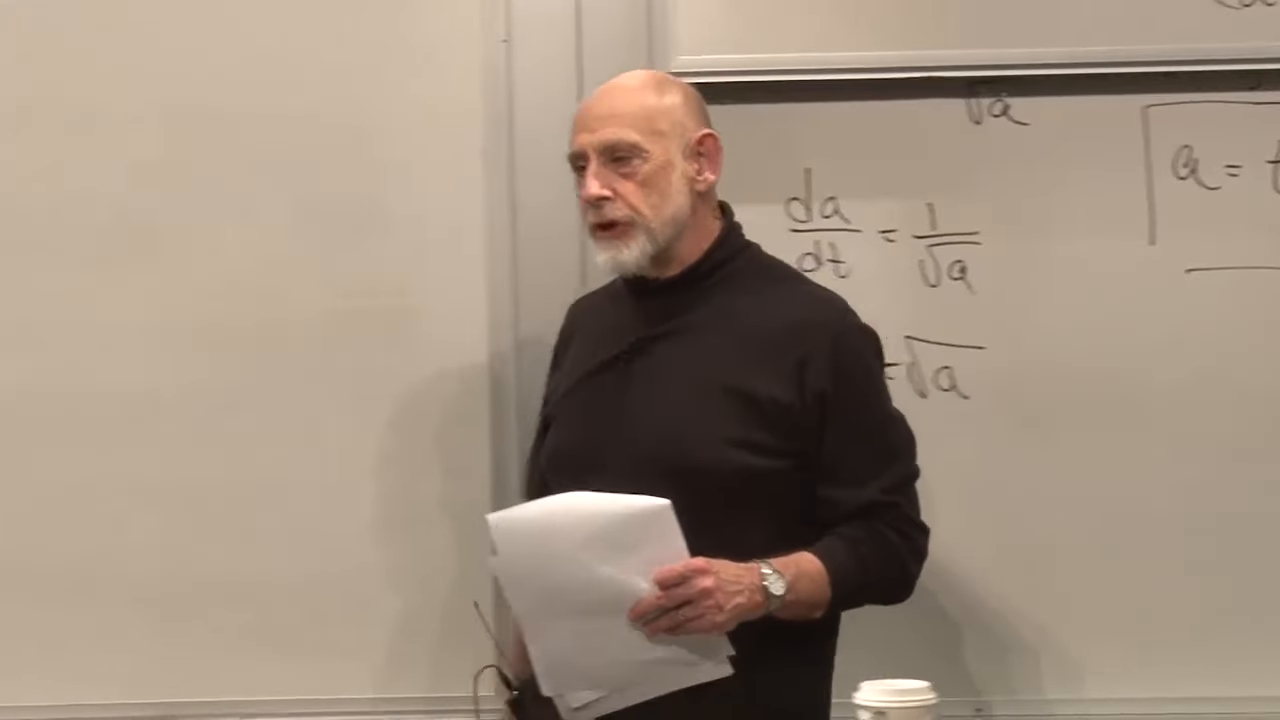
\includegraphics[width=0.68\textwidth]{lecture_02_figure_02.png}
\caption{Le tableau récapitulatif consigne \(\dot a=1/\sqrt a\) ainsi que la loi encadrée pour un univers dominé par la matière \(a\propto t^{2/3}\). Une partie de l’algèbre intermédiaire est masquée ; les équations~\eqref{eq:c02-zero-energy-friedmann}--\eqref{eq:c02-matter-law} la fournissent.}
\label{fig:c02-matter-recap}
\lectureframe{00:29:20.838}
\end{figure}

\begin{classroomqa}
\audiencequestion{Pourquoi a-t-on écarté la racine carrée négative ?}
\lecturerresponse{L’équation ne l’écarte pas. L’équation~\eqref{eq:c02-zero-energy-friedmann} fixe \(H^2\), mais pas le signe de \(H\). La racine positive décrit l’expansion, et la racine négative la contraction. Une pierre dans le champ gravitationnel d’une planète peut se déplacer vers l’extérieur ou vers l’intérieur tout en satisfaisant la même équation de l’énergie ; c’est la condition initiale qui détermine la branche. Nous avons choisi la branche en expansion parce que c’est celle de l’univers considéré ici. \lecturetimestamp{00:23:09--00:24:46}}
\end{classroomqa}

Le modèle suivant continuera à négliger l’énergie noire. Cette omission est délibérée : nous allons d’abord comprendre le cadre ancien matière-rayonnement avant d’ajouter la composante qui gouverne l’époque actuelle d’expansion accélérée. En revanche, la matière noire est déjà incluse dans le terme de matière, car elle aussi, lorsqu’elle est non relativiste, se dilue comme \(a^{-3}\).

\begin{classroomqa}
\audiencequestion{L’énergie noire n’est-elle pas la composante dominante aujourd’hui ?}
\lecturerresponse{Si. Le scénario à deux composantes présenté ici correspond à la cosmologie pédagogique standard d’avant la découverte de l’accélération actuelle. La matière noire est incluse dans la matière ; l’énergie noire constitue une troisième composante, qui sera introduite séparément. Partir de l’ancien modèle permet de voir ce que modifie chaque terme supplémentaire. \lecturetimestamp{00:28:02--00:28:45}}
\end{classroomqa}

\section{Rétablir la constante d’énergie}

Le choix d’une énergie nulle est une condition initiale particulière. Pour l’abandonner, considérons une galaxie de masse \(m\) située à la limite d’une sphère homogène. Soit \(x\) son rayon comobile, de sorte que
\begin{equation}
D=ax,
\qquad
\dot D=\dot a x.
\label{eq:c02-comoving-particle}
\end{equation}
Le théorème des coquilles de Newton stipule que seule la masse \(M(D)\) contenue dans la sphère contribue à l’accélération radiale ; les coquilles sphériques extérieures n’exercent aucune force nette. L’énergie newtonienne conservée de la galaxie vaut
\begin{equation}
\frac{1}{2}m\dot D^{\,2}-\frac{GM(D)m}{D}=E.
\label{eq:c02-newton-energy}
\end{equation}
Le facteur \(m\) doit figurer dans les deux termes. On peut facilement l’omettre en écrivant rapidement au tableau, mais le conserver montre clairement que la constante finale est l’énergie par unité de masse de la particule test.

L’homogénéité nous permet de choisir la galaxie représentative en \(x=1\). On a alors \(D=a\), \(\dot D=\dot a\), et la sphère a pour
\begin{equation}
V_{\rm sph}=\frac{4\pi}{3}a^3,
\qquad
M(a)=\rho_m V_{\rm sph}=\frac{4\pi}{3}\rho_m a^3.
\label{eq:c02-enclosed-mass}
\end{equation}
Au tableau, le symbole \(V\) sert à la fois pour le volume et, dans une annotation latérale, pour la vitesse radiale. Nous utiliserons les symboles sans ambiguïté \(V_{\rm sph}\) et \(\dot D\).

\begin{figure}[ht]
\centering
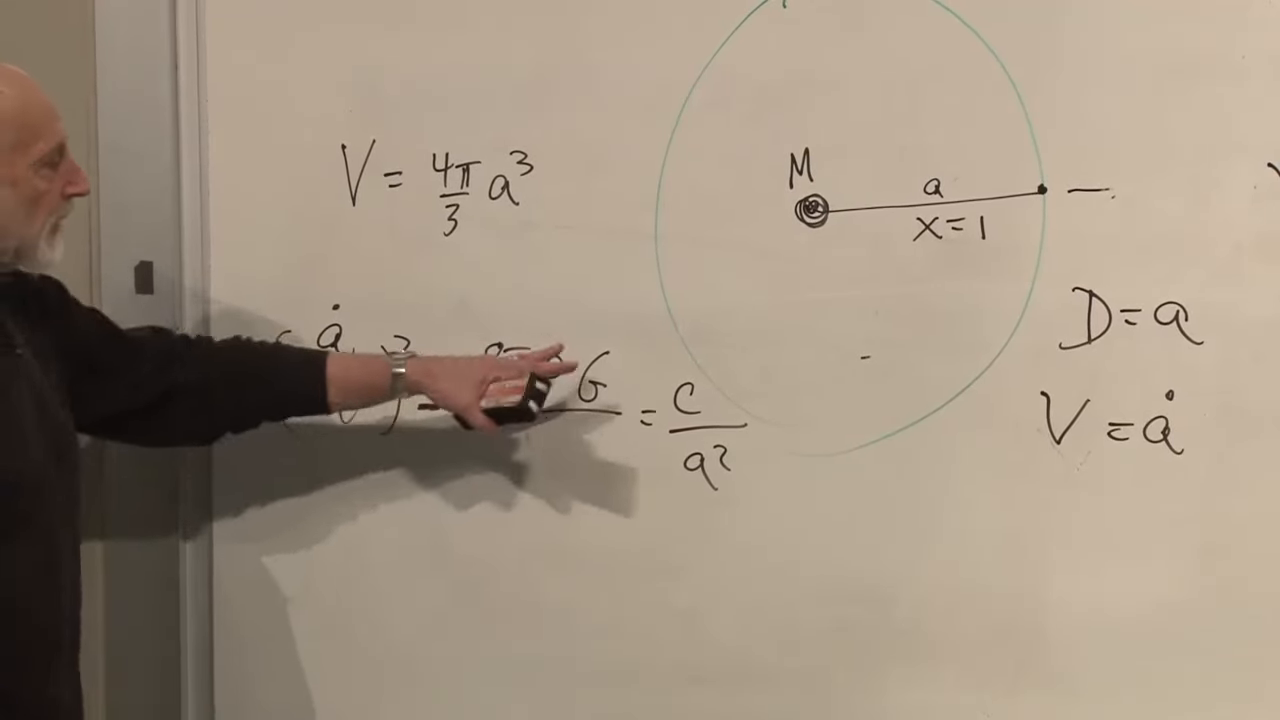
\includegraphics[width=0.86\textwidth]{lecture_02_figure_03.png}
\caption{La sphère de masse intérieure et l’équation de Friedmann pour une énergie non nulle. Les indications visibles comprennent \(V_{\rm sph}=4\pi a^3/3\), la masse centrale \(M\), \(x=1\), \(D=a\) et \(\dot D=\dot a\). Le chargé de cours masque une partie de l’équation, que l’on reconstitue algébriquement ci-dessous.}
\label{fig:c02-energy-board}
\lectureframe{00:37:59.876}
\end{figure}

\begin{figure}[ht]
\centering
\begin{tikzpicture}[scale=1.05,>=Latex]
  \draw[thick] (0,0) circle (2.6);
  \fill (0,0) circle (2.2pt) node[below left=2pt] {\(M(a)\)};
  \draw[thick,->] (0,0) -- (2.58,0);
  \fill (2.6,0) circle (2.2pt) node[right=4pt] {galaxy \(m\)};
  \node[above] at (1.30,0.04) {\(D=ax\)};
  \node[below] at (1.30,-0.04) {\(x=1\Rightarrow D=a\)};
  \draw[->,blue!60!black,thick] (2.63,0.18) -- (3.55,0.72)
    node[right] {\(\dot D=\dot a\)};
  \node at (0,-3.05) {\(M(a)=\frac{4\pi}{3}\rho_m a^3\)};
\end{tikzpicture}
\caption{Reconstitution claire de la sphère newtonienne en \(x=1\). Les coquilles extérieures s’annulent ; la galaxie située à la limite ne réagit donc qu’à la masse intérieure.}
\label{fig:c02-sphere-redraw}
\end{figure}

Substituons \(D=a\) dans l’équation~\eqref{eq:c02-newton-energy}, divisons par \(m/2\) et définissons la constante
\begin{equation}
C\equiv\frac{2E}{m}.
\end{equation}
On obtient
\begin{equation}
\dot a^{\,2}-\frac{2GM(a)}{a}=C.
\label{eq:c02-energy-a}
\end{equation}
En divisant par \(a^2\) et en utilisant l’équation~\eqref{eq:c02-enclosed-mass}, on trouve
\begin{equation}
\left(\frac{\dot a}{a}\right)^2-
\frac{8\pi G}{3}\rho_m=\frac{C}{a^2},
\label{eq:c02-energy-form}
\end{equation}
ou, de manière équivalente,
\begin{equation}
\boxed{H^2=\frac{8\pi G}{3}\rho_m+\frac{C}{a^2}.}
\label{eq:c02-friedmann-C}
\end{equation}
C’est la première équation de Friedmann pour de la matière sans pression, écrite selon la convention newtonienne de l’énergie. Le nouveau terme \(a^{-2}\) conserve la mémoire du fait que la galaxie représentative a été lancée au-dessus, à la valeur ou en dessous de l’énergie d’échappement.

En substituant \(\rho_m=\nu_m/a^3\), il est commode de définir
\begin{equation}
A_m\equiv\frac{8\pi G\nu_m}{3}>0,
\end{equation}
de sorte que
\begin{equation}
H^2=\frac{A_m}{a^3}+\frac{C}{a^2},
\qquad
\dot a^{\,2}=\frac{A_m}{a}+C.
\label{eq:c02-energy-branches}
\end{equation}
L’équation est plus instructive si on la lit en considérant ses limites que si on l’intègre immédiatement.

\subsection{Énergie positive}

Si \(C>0\), le terme de matière \(A_m/a^3\) domine aux petites valeurs de \(a\). L’expansion initiale suit donc toujours la loi de matière \(a\propto t^{2/3}\). Aux grandes valeurs de \(a\), en revanche, le terme \(C/a^2\) domine dans \(H^2\), ou, de manière équivalente,
\begin{equation}
\dot a^{\,2}\longrightarrow C.
\end{equation}
L’expansion tend vers une vitesse constante,
\begin{equation}
a(t)\sim\sqrt C\,t.
\label{eq:c02-positive-late}
\end{equation}
C’est l’équivalent cosmologique du lancer d’une pomme à une vitesse supérieure à la vitesse d’échappement. La gravité réduit continuellement sa vitesse, mais, loin de la planète, la pomme conserve une vitesse asymptotique non nulle.

\subsection{Énergie nulle}

Pour \(C=0\), l’équation~\eqref{eq:c02-energy-branches} redonne la solution critique \(a\propto t^{2/3}\). L’expansion se poursuit sans limite tandis que \(\dot a\) tend vers zéro. C’est le cas exact de l’énergie d’échappement.

\subsection{Énergie négative}

Si \(C=-|C|<0\), alors
\begin{equation}
H^2=\frac{A_m}{a^3}-\frac{|C|}{a^2}
=\frac{A_m-|C|a}{a^3}.
\label{eq:c02-negative-energy}
\end{equation}
Le facteur d’échelle ne peut dépasser
\begin{equation}
a_{\max}=\frac{A_m}{|C|},
\label{eq:c02-amax}
\end{equation}
car le membre de droite s’y annule. La branche en expansion atteint \(a_{\max}\) avec \(\dot a=0\) ; la suite correspond à la branche en contraction. Dans l’image newtonienne, c’est une pomme lancée à une vitesse inférieure à la vitesse d’échappement : elle monte, rebrousse chemin et retombe.

\begin{classroomqa}
\audiencequestion{Comment le modèle peut-il décrire un effondrement si le membre de droite est égal à \(H^2\) et ne peut donc pas être négatif ?}
\lecturerresponse{Il ne devient jamais négatif. Au cours de l’expansion, le membre de droite décroît jusqu’à s’annuler en \(a_{\max}\). Là, \(H=0\). La solution passe alors de la racine carrée positive à la racine carrée négative et retrace la région permise avec \(\dot a<0\). On pourrait être tenté de prolonger l’évolution de façon incorrecte en laissant l’expression traverser zéro. C’est impossible : zéro est la limite de la région permise, et non une valeur que \(H\) pourrait traverser tout en restant réel. \lecturetimestamp{00:48:43--00:53:03}}
\end{classroomqa}

Les trois valeurs de l’énergie newtonienne donnent donc trois histoires qualitativement distinctes : effondrement pour \(C<0\), échappement critique pour \(C=0\) et expansion éternelle à \(\dot a\) asymptotiquement constante pour \(C>0\). L’étape suivante, surprenante, est que la relativité générale attribue à ces mêmes cas une signification géométrique.

\section{De l’énergie à la courbure}

Dans l’équation~\eqref{eq:c02-friedmann-C}, plaçons le terme d’énergie du côté géométrique et définissons
\begin{equation}
k\equiv-C.
\label{eq:c02-k-definition}
\end{equation}
On obtient alors
\begin{equation}
\boxed{H^2+\frac{k}{a^2}=\frac{8\pi G}{3}\rho.}
\label{eq:c02-friedmann-k}
\end{equation}
Au tableau, les notations \(C\), \(K\) et \(\kappa\) alternent, et un signe est absorbé lorsque le terme passe de l’autre côté de l’égalité. L’équation~\eqref{eq:c02-k-definition} fixe notre convention : une énergie newtonienne positive correspond à \(k<0\), une énergie nulle à \(k=0\), et une énergie négative à \(k>0\).

\begin{figure}[ht]
\centering
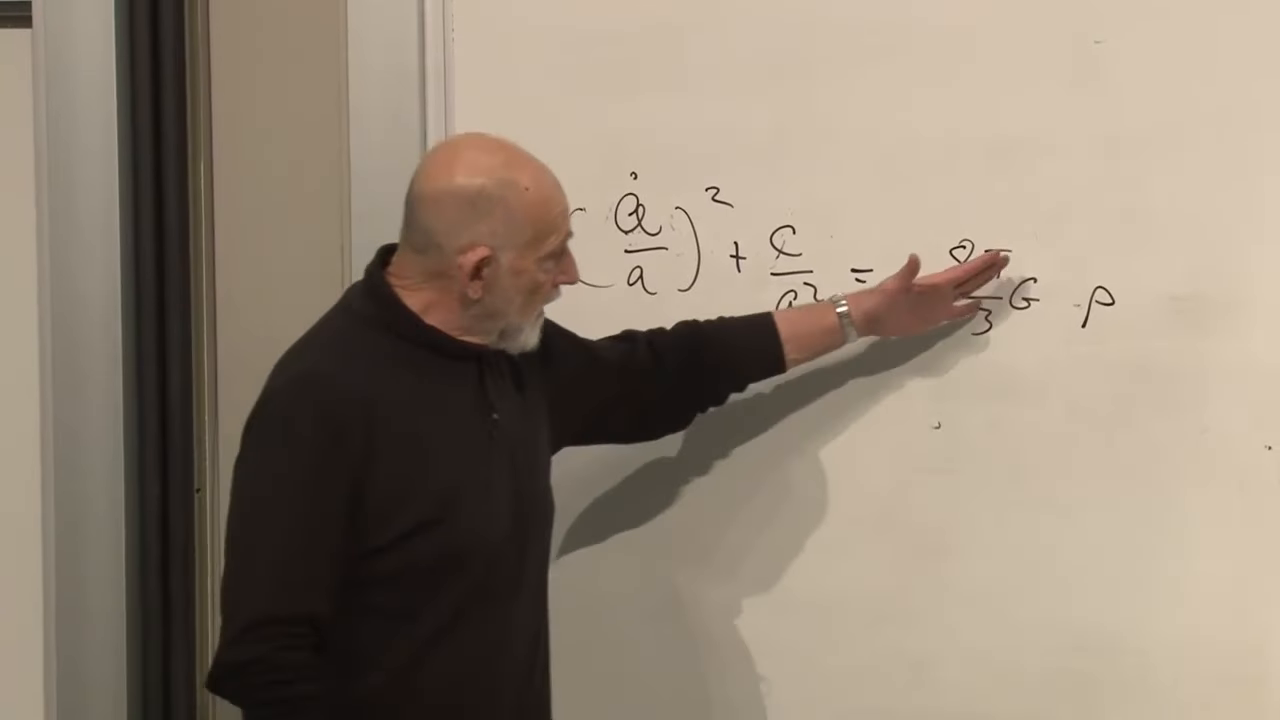
\includegraphics[width=0.76\textwidth]{lecture_02_figure_04.png}
\caption{L’équation de Friedmann écrite avec la géométrie à gauche et la source à droite. Le tableau illustre cette division conceptuelle ; il ne présente pas l’équation tensorielle complète d’Einstein.}
\label{fig:c02-geometry-source}
\lectureframe{00:55:22.810}
\end{figure}

Cette écriture est une version miniature de l’équation d’Einstein. Le membre de gauche décrit la géométrie : l’expansion par \(H\) et la courbure spatiale par \(k/a^2\). Le membre de droite décrit la source matérielle. En mécanique newtonienne, cette source était la densité de masse. En relativité, il s’agit de l’énergie et de la quantité de mouvement, représentées dans leur totalité par le tenseur énergie-impulsion. Pour un univers homogène et isotrope, la première équation de Friedmann dépend de la densité totale d’énergie \(\rho\).

Si l’on conserve les unités ordinaires, la densité de masse contribue par son énergie au repos \(\rho_{\rm mass}c^2\). À partir d’ici, nous posons \(c=1\), de sorte que masse et énergie s’expriment dans les mêmes unités. Le symbole \(\rho\) peut alors inclure la masse au repos, l’énergie cinétique, le rayonnement et toute autre composante homogène de l’énergie.

\begin{figure}[ht]
\centering
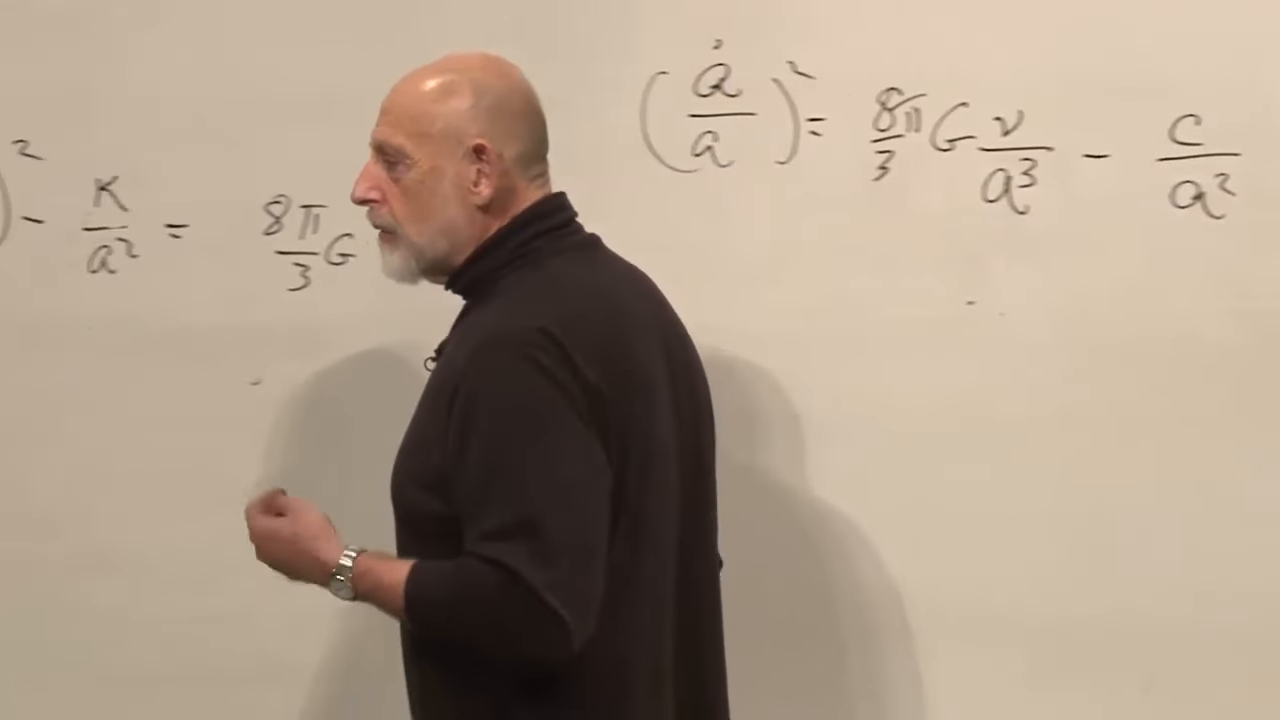
\includegraphics[width=0.88\textwidth]{lecture_02_figure_05.png}
\caption{Formes côte à côte de l’équation de Friedmann inscrites au tableau : une forme faisant intervenir la courbure avec \(\rho\), et une forme pour la matière obtenue après \(\rho_m=\nu_m/a^3\). La notation change au tableau ; l’équation~\eqref{eq:c02-k-definition} conserve la convention de signe fixée ici.}
\label{fig:c02-curvature-comparison}
\lectureframe{00:57:52.659}
\end{figure}

L’interprétation géométrique est globale. Dans le modèle relativiste, \(k=0\) décrit des tranches spatiales plates, \(k>0\) des tranches sphériques à courbure positive et \(k<0\) des tranches hyperboliques à courbure négative. La dérivation newtonienne a reproduit la même équation d’évolution sans comporter ces géométries globales. Sa constante d’énergie non nulle imite donc la courbure avec une remarquable précision, mais ne dérive pas l’espace courbe lui-même.

\begin{classroomqa}
\audiencequestion{Comment la mécanique newtonienne et la relativité générale peuvent-elles produire la même équation d’expansion si leurs géométries sont différentes ?}
\lecturerresponse{La relativité générale inclut le cas plat et, localement, toute géométrie régulière est approximativement plate. Plus remarquable encore, la constante d’énergie newtonienne intervient dans l’équation d’évolution exactement à la place occupée par la courbure spatiale relativiste. La formule dynamique est la même, mais l’interprétation globale ne l’est pas : l’espace euclidien newtonien ne s’est pas secrètement transformé en espace sphérique ou hyperbolique. Il faudra construire ces trois géométries dans le cadre de la relativité générale. \lecturetimestamp{01:20:59--01:24:20}}
\end{classroomqa}

\section{Le rayonnement dans une boîte en expansion}

Changeons maintenant le contenu de l’Univers. Considérons un cube comobile d’unité de côté. Son volume physique est \(a^3\). Pour la matière non relativiste, le nombre de particules dans cette boîte est fixe et l’énergie au repos de chaque particule est approximativement constante, d’où \(\rho_m\propto a^{-3}\). Le rayonnement subit un effet supplémentaire : chaque photon perd de l’énergie à mesure que l’Univers se dilate.

Un photon de longueur d’onde \(\lambda\) a pour énergie
\begin{equation}
E_\gamma=\frac{hc}{\lambda},
\qquad
E_\gamma\propto\lambda^{-1}.
\label{eq:c02-photon-energy}
\end{equation}
Dans une expansion homogène, la longueur d’onde d’une onde en propagation libre s’étire avec le facteur d’échelle :
\begin{equation}
\frac{\lambda(t_2)}{\lambda(t_1)}
=\frac{a(t_2)}{a(t_1)},
\qquad
\lambda\propto a.
\label{eq:c02-redshift}
\end{equation}
C’est le décalage cosmologique vers le rouge. Il en découle
\begin{equation}
E_\gamma\propto a^{-1}.
\label{eq:c02-photon-redshift}
\end{equation}
Si le nombre de photons dans la boîte comobile se conserve, l’énergie totale du rayonnement diminue comme \(a^{-1}\). En divisant par le volume physique \(a^3\), on obtient
\begin{equation}
\boxed{\rho_r(a)=\frac{\nu_r}{a^4}.}
\label{eq:c02-radiation-density}
\end{equation}
Ici, \(\nu_r\) est l’amplitude constante de la densité de rayonnement en propagation libre. Le rayonnement comporte une puissance inverse supplémentaire de \(a\) par rapport à la matière : trois puissances dues à la dilution spatiale, et une due au décalage vers le rouge de chaque photon.

L’analogie avec une corde de guitare donne une intuition utile. Un mode qui s’établit sur une corde comporte un nombre entier de demi-longueurs d’onde. Si l’on allonge lentement la corde, ce nombre ne peut pas varier de façon continue ; c’est plutôt la longueur d’onde qui s’ajuste à la nouvelle longueur. De même, pour une onde sur un anneau qui se dilate lentement, le nombre de nœuds est un invariant adiabatique et sa longueur d’onde suit la circonférence. Toute onde peut être décomposée en de tels modes.

Cela ne remplace pas la résolution des équations de Maxwell dans un espace-temps en expansion. C’est l’intuition contrôlée qui sous-tend l’équation~\eqref{eq:c02-redshift} : l’expansion lente de la géométrie modifie la longueur d’onde physique tout en préservant l’étiquette du mode.

\begin{classroomqa}
\audiencequestion{Cet argument suppose-t-il une boîte conductrice ou réfléchissante ? Que se passe-t-il dans un espace en expansion vide, sans parois matérielles ?}
\lecturerresponse{Les parois servent de dispositif de comptabilité ; elles ne signifient pas que l’Univers est enfermé dans une enceinte conductrice. Une démonstration complète découle de la propagation des ondes dans la métrique en expansion. Pour l’argument présent, nous nous appuyons sur le fait observé et dérivé en relativité que les longueurs d’onde en propagation libre évoluent comme \(a\). La boîte aide à compter les photons et le volume physique ; elle n’est pas à l’origine du décalage cosmologique vers le rouge. \lecturetimestamp{01:02:21--01:04:37}}
\end{classroomqa}

\begin{classroomqa}
\audiencequestion{Pourquoi la longueur d’onde suit-elle la grille au lieu de conserver une longueur physique fixe ?}
\lecturerresponse{Considérons un mode sur un anneau dont la circonférence varie de façon adiabatique. Son nombre entier de nœuds ne peut pas dériver continûment ; la longueur d’onde autorisée doit donc varier avec celle de l’anneau. Le développement d’une onde générale en modes de Fourier mène à la même conclusion, mode par mode. Cela fournit l’intuition adiabatique nécessaire ; l’énoncé exact relève de la théorie des champs en espace-temps courbe. \lecturetimestamp{01:34:18--01:38:33}}
\end{classroomqa}

\subsection{La solution dominée par le rayonnement}

En négligeant provisoirement la courbure, introduisons l’équation~\eqref{eq:c02-radiation-density} dans l’équation de Friedmann :
\begin{equation}
H^2=\frac{8\pi G\nu_r}{3a^4}
\equiv\frac{A_r}{a^4},
\qquad A_r>0.
\label{eq:c02-radiation-friedmann}
\end{equation}
Sur la branche en expansion,
\begin{equation}
\frac{\dot a}{a}=\frac{\sqrt{A_r}}{a^2},
\qquad
\dot a=\frac{\sqrt{A_r}}{a}.
\end{equation}
On a donc
\begin{equation}
a\,da=\sqrt{A_r}\,dt,
\qquad
\frac{a^2}{2}=\sqrt{A_r}(t-t_B),
\end{equation}
puis
\begin{equation}
\boxed{a(t)\propto(t-t_B)^{1/2}.}
\label{eq:c02-radiation-law}
\end{equation}
La différence entre les exposants \(1/2\) et \(2/3\) paraît modeste visuellement, mais elle est décisive physiquement. Le taux d’expansion, la température, le gel des réactions et la taille de l’horizon dans l’Univers primordial dépendent tous de la composante dominante.

\section{Un univers de matière et de rayonnement}

Pour la matière et le rayonnement conservés séparément, leurs densités s’additionnent :
\begin{equation}
\rho(a)=\rho_m(a)+\rho_r(a).
\end{equation}
En négligeant la courbure pour cette comparaison,
\begin{equation}
\boxed{H^2=\frac{C_m}{a^3}+\frac{C_r}{a^4},}
\label{eq:c02-mixed-friedmann}
\end{equation}
où \(C_m,C_r>0\). Au tableau, les deux coefficients sont d’abord notés \(C_1\) et \(C\) ; le second symbole est ensuite corrigé verbalement et désigne une constante distincte. La notation de l’équation~\eqref{eq:c02-mixed-friedmann} explicite cette correction.

\begin{figure}[ht]
\centering
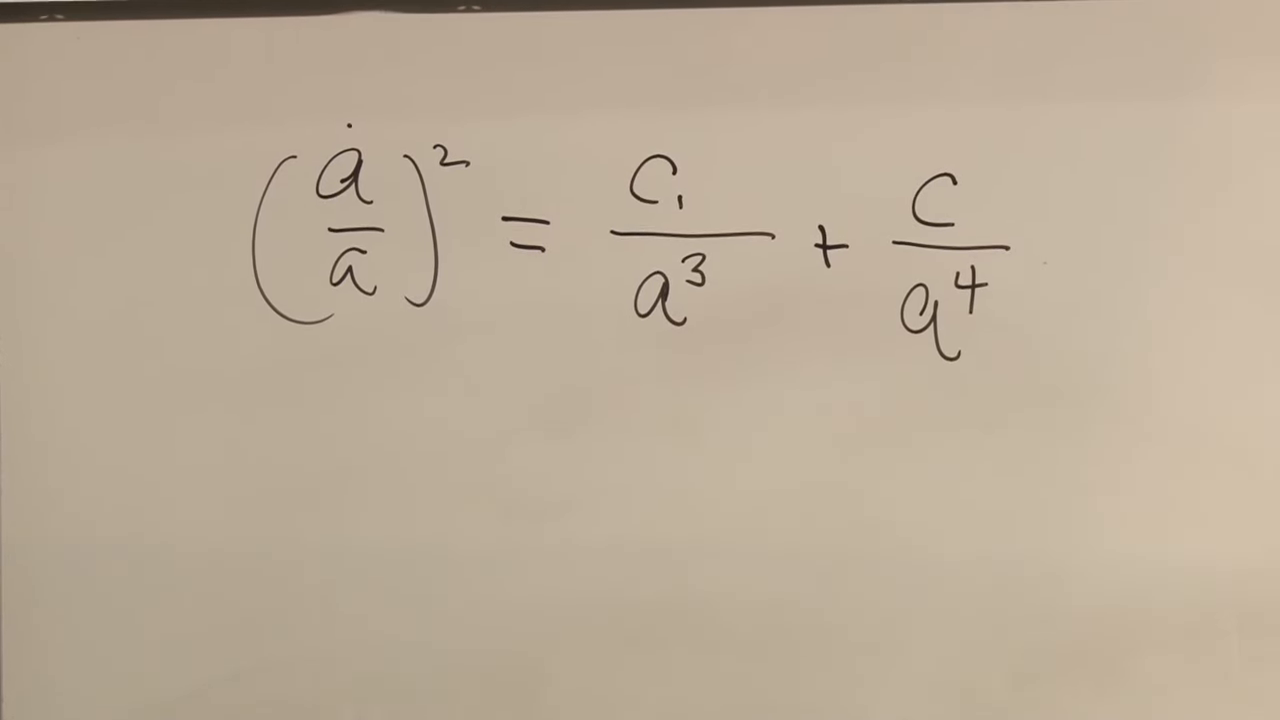
\includegraphics[width=0.74\textwidth]{lecture_02_figure_06.png}
\caption{L’équation mêlant matière et rayonnement inscrite au tableau. Le second coefficient écrit est ensuite corrigé et remplacé par une constante propre au rayonnement, notée \(C_r\) dans l’équation~\eqref{eq:c02-mixed-friedmann}.}
\label{fig:c02-mixed-board}
\lectureframe{01:11:37.997}
\end{figure}

Aux petites valeurs de \(a\), le terme de rayonnement l’emporte, car \(a^{-4}\) croît plus vite que \(a^{-3}\) :
\begin{equation}
a\ll a_{\rm eq}
\quad\Longrightarrow\quad
H^2\simeq\frac{C_r}{a^4},
\qquad
a(t)\propto t^{1/2}.
\end{equation}
Aux valeurs plus grandes de \(a\), la matière l’emporte :
\begin{equation}
a\gg a_{\rm eq}
\quad\Longrightarrow\quad
H^2\simeq\frac{C_m}{a^3},
\qquad
a(t)\propto t^{2/3}.
\end{equation}
L’échelle d’égalité s’obtient directement en égalant les deux termes :
\begin{equation}
a_{\rm eq}=\frac{C_r}{C_m}.
\label{eq:c02-equality-scale}
\end{equation}
Cette égalité ne correspond pas au même événement que le découplage des photons. L’égalité désigne l’instant où les deux densités d’énergie sont identiques ; le découplage, celui où les interactions cessent de maintenir la matière et le rayonnement en contact thermique.

Le secteur du rayonnement comprend les photons et toutes les espèces se déplaçant de façon ultrarelativiste. Les neutrinos très légers se comportent ainsi lorsque la température est suffisamment élevée, et un fond de gravitons évoluerait de la même manière. Lorsqu’une espèce massive devient non relativiste, sa contribution dominante, liée à la masse au repos, commence à évoluer comme la matière. La matière noire froide appartient à \(C_m/a^3\), et non au terme de rayonnement.

\begin{classroomqa}
\classquestion{Quel terme de l’équation~\eqref{eq:c02-mixed-friedmann} domine d’abord, et lequel domine plus tard ?}
\lecturerresponse{Pour les petites valeurs de \(a\), \(a^{-4}\) l’emporte sur \(a^{-3}\) : le rayonnement gouverne donc l’expansion initiale et donne \(a\propto t^{1/2}\). À mesure que \(a\) augmente, le rapport rayonnement-matière décroît comme \(1/a\) ; la matière gouverne alors l’expansion et donne \(a\propto t^{2/3}\). \lecturetimestamp{01:11:46--01:13:38}}
\end{classroomqa}

\begin{classroomqa}
\audiencequestion{Suppose-t-on que les proportions relatives de matière et de rayonnement restent constantes ?}
\lecturerresponse{Leurs densités ne sont pas constantes, mais on peut traiter les coefficients \(C_m\) et \(C_r\) comme constants une fois que les composantes cessent d’échanger efficacement de l’énergie et que la création ou l’annihilation de particules devient négligeable. La matière conserve alors une masse au repos comobile, et le rayonnement libre un nombre de photons comobile ; le décalage vers le rouge lui apporte son facteur supplémentaire de \(a^{-1}\). Durant les périodes d’interactions fortes ou d’annihilation d’espèces, il faut affiner ce bilan. \lecturetimestamp{01:13:39--01:14:53}}
\end{classroomqa}

\begin{classroomqa}
\audiencequestion{À quel moment la matière et le rayonnement ont-ils cessé d’interagir fortement ?}
\lecturerresponse{Un ordre de grandeur approximatif est de \(10^5\) ans pour le découplage des photons de la matière ordinaire. L’histoire précise de la recombinaison relève d’un calcul ultérieur et ne doit pas être confondue avec l’égalité matière--rayonnement. Pour notre propos, il suffit de retenir qu’après le découplage on peut suivre approximativement les deux composantes séparément. \lecturetimestamp{01:27:29--01:27:46}}
\end{classroomqa}

\begin{classroomqa}
\audiencequestion{Comment savoir qu’il y a eu une époque précoce où \(a\propto t^{1/2}\), avant même l’existence des galaxies qui pourraient servir à suivre l’expansion ?}
\lecturerresponse{Nous déduisons l’histoire de l’expansion des traces physiques qu’elle a laissées. La nucléosynthèse primordiale dépend de la compétition précoce entre les taux de réaction et \(H(t)\) ; le fond diffus cosmologique témoigne de l’état thermique ultérieur et des perturbations. Les observations des galaxies rendent le comportement de l’ère de la matière plus directement accessible, tandis que l’ère du rayonnement est reconstituée à partir de ces indices sur l’Univers primordial. \lecturetimestamp{01:27:46--01:30:10}}
\end{classroomqa}

Le modèle matière-rayonnement est délibérément incomplet. C’est le cadre classique dans lequel l’Univers passe d’une domination du rayonnement à une domination de la matière. L’expansion accélérée actuelle requiert une autre source, l’énergie noire, qui ajoutera un terme d’une nature qualitativement différente.

\section{Où va l’énergie décalée vers le rouge ?}

La diminution \(E_\gamma\propto a^{-1}\) soulève une question inévitable : où est passée l’énergie des photons ? Dans une boîte réelle à parois réfléchissantes en expansion, le rayonnement exerce une pression et effectue un travail sur les parois. La relation thermodynamique s’écrit
\begin{equation}
dE=-p\,dV.
\label{eq:c02-pdv}
\end{equation}
À mesure que \(V\) augmente, l’énergie du rayonnement diminue. L’énergie perdue peut se retrouver sous forme d’énergie cinétique, de contrainte ou de chaleur dans ce qui déplace les parois.

La boîte comobile n’a pas de parois matérielles. C’est une frontière imaginaire qui se déplace avec l’expansion moyenne. Les photons la traversent, mais, dans un bain de rayonnement homogène, le flux statistique entrant compense le flux sortant. La boîte reste un volume de référence valide, même si ce n’est pas un récipient. La loi du travail de pression décrit toujours l’évolution de l’énergie contenue dans un volume comobile.

Pour le rayonnement, \(p=\rho/3\) et \(E=\rho V\). L’équation~\eqref{eq:c02-pdv} donne alors
\begin{align}
d(\rho V)&=-\frac{\rho}{3}\,dV,\\
V\,d\rho&=-\frac{4}{3}\rho\,dV,\\
\frac{d\rho}{\rho}&=-\frac{4}{3}\frac{dV}{V}.
\end{align}
Puisque \(V\propto a^3\), l’intégration donne \(\rho\propto a^{-4}\), conformément à l’argument fondé sur la longueur d’onde. Cette dérivation thermodynamique montre également que l’énergie de chaque photon diminue, et pas seulement la densité numérique.

\begin{classroomqa}
\audiencequestion{Où va l’énergie des photons décalés vers le rouge ? L’énergie totale de l’Univers se conserve-t-elle ?}
\lecturerresponse{Avec des parois matérielles, le rayonnement leur fournit du travail : le bilan relève alors de la mécanique ordinaire. Pour l’Univers dans son ensemble, la question est plus subtile. La conservation globale de l’énergie découle normalement de la symétrie par translation dans le temps ; or un espace-temps en expansion n’est généralement pas invariant sous une telle translation et ne possède pas nécessairement une énergie totale conservée qui soit définie de manière unique. On peut construire des analogies newtoniennes utiles faisant intervenir l’énergie de l’expansion, mais toute conclusion définitive à l’échelle globale exige la relativité générale. Les deux descriptions sont utiles ici, mais le modèle newtonien ne permet pas de trancher définitivement la question globale. \lecturetimestamp{01:16:51--01:20:58}}
\end{classroomqa}

\begin{classroomqa}
\audiencequestion{Si la boîte comobile est imaginaire et que les photons franchissent sa frontière, en quoi l’image du travail de pression reste-t-elle utile ?}
\lecturerresponse{L’homogénéité fournit le bilan manquant. En moyenne, chaque photon qui quitte un volume comobile est statistiquement remplacé par un photon venant du volume voisin. Les flux locaux se compensent en moyenne, tandis que le volume physique et les longueurs d’onde changent. Une boîte réfléchissante rend concret le mécanisme du travail ; la boîte comobile décrit la même loi de conservation moyenne sans parois réelles. \lecturetimestamp{01:24:22--01:27:28}}
\end{classroomqa}

\begin{classroomqa}
\audiencequestion{L’expansion ne fait-elle que réduire la densité de photons, ou réduit-elle aussi l’énergie de chaque photon ?}
\lecturerresponse{Les deux phénomènes se produisent. Le nombre de photons par unité de volume physique diminue comme \(a^{-3}\), et le décalage cosmologique vers le rouge réduit l’énergie de chaque photon d’un facteur supplémentaire \(a^{-1}\). C’est l’équivalent radiatif du refroidissement adiabatique. Un gaz ordinaire se refroidit lui aussi en effectuant un travail lors d’une expansion lente, même si une détente libre brutale relève d’un autre processus thermodynamique. \lecturetimestamp{01:42:30--01:45:55}}
\end{classroomqa}

\section{Récession, horizons et limites du modèle}

La loi de Hubble associe la vitesse de récession
\begin{equation}
v_{\rm rec}=HD
\label{eq:c02-recession}
\end{equation}
à un objet situé à la distance propre \(D\) sur une tranche de temps cosmique donnée. Pour des valeurs suffisamment grandes de \(D\), l’équation~\eqref{eq:c02-recession} peut donner une valeur supérieure à \(c\). Cela ne viole pas la relativité restreinte, car \(v_{\rm rec}\) n’est pas la vitesse d’un objet proche mesurée dans un même référentiel inertiel local. Elle compare des lignes d’univers comobiles très éloignées dans une géométrie qui évolue. Tout observateur local mesure toujours la vitesse de la lumière comme étant \(c\), et aucun objet matériel local ne dépasse un autre objet à une vitesse supérieure à celle de la lumière.

\begin{classroomqa}
\audiencequestion{Une galaxie suffisamment éloignée peut-elle s’éloigner à une vitesse supérieure à celle de la lumière ?}
\lecturerresponse{Oui, sa vitesse cosmologique de récession \(HD\) peut dépasser \(c\). Aucun objet local ne dépasse alors un observateur voisin à une vitesse supérieure à celle de la lumière, et ce résultat ne peut pas servir à transmettre des signaux supraluminiques. Il s’agit de l’évolution de la distance propre entre des lignes d’univers comobiles éloignées, et non d’une vitesse ordinaire de la relativité restreinte mesurée en un événement. \lecturetimestamp{01:30:17--01:32:13}}
\end{classroomqa}

Le fait qu’une galaxie s’éloigne à une vitesse supraluminique ne permet pas, à lui seul, de savoir si la lumière qu’elle émet maintenant nous parviendra un jour. Cela dépend de toute l’histoire future de l’expansion. Dans un modèle dominé par la matière et en décélération, des régions qui s’éloignent actuellement à une vitesse supérieure à celle de la lumière peuvent devenir observables par la suite, car l’horizon pertinent évolue. Si l’expansion accélérée se poursuit, un horizon des événements peut cacher définitivement les événements suffisamment éloignés.

\begin{classroomqa}
\audiencequestion{Les galaxies disparaissent-elles dès que leur vitesse de récession dépasse celle de la lumière ?}
\lecturerresponse{Pas nécessairement. Le franchissement du rayon de Hubble et l’existence d’un véritable horizon des événements sont deux notions différentes. Dans un modèle en décélération, la lumière provenant d’une région qui s’éloigne actuellement à une vitesse supraluminique peut tout de même nous parvenir plus tard. Une domination persistante de l’énergie noire modifie la structure causale globale et peut créer un horizon ultime. Pour déterminer quels signaux nous parviennent, il faut connaître la géométrie de l’espace-temps, et pas seulement une valeur instantanée de \(HD\). \lecturetimestamp{01:32:14--01:34:18}}
\end{classroomqa}

Le langage de la relativité restreinte peut également induire en erreur lorsqu’on l’applique à l’échelle globale. La masse au repos invariante d’une particule n’augmente pas avec sa vitesse. Son énergie et sa quantité de mouvement dépendent du référentiel local de l’observateur. Les particules massives ne peuvent pas être accélérées jusqu’à dépasser la vitesse locale de la lumière, mais la récession d’une galaxie comobile éloignée ne correspond pas à son passage dans un référentiel local unique.

\begin{classroomqa}
\audiencequestion{Une galaxie qui s’éloigne rapidement acquiert-elle une masse relativiste plus grande ?}
\lecturerresponse{Il est préférable d’éviter le terme ``masse relativiste.'' La galaxie possède une masse au repos invariante, tandis que son énergie et sa quantité de mouvement dépendent du référentiel. De plus, une vitesse de récession attribuée sur une distance cosmologique n’est pas la vitesse locale qui intervient dans la formule de la relativité restreinte. Ces notions ne concordent que si l’on compare les événements éloignés à l’aide de la métrique de l’espace-temps. \lecturetimestamp{01:38:34--01:40:05}}
\end{classroomqa}

\begin{classroomqa}
\audiencequestion{Que deviennent les axes du temps et de l’espace lorsque la vitesse de récession d’une galaxie éloignée est supraluminique ?}
\lecturerresponse{Il n’existe pas de référentiel de Lorentz global unique dont les axes inclinés permettraient de trancher la question. La relativité restreinte compare des référentiels inertiels dans un espace-temps plat ; la cosmologie exige une métrique qui relie les référentiels locaux sur un espace-temps courbe étendu. Le raisonnement newtonien reste fiable dans une petite région, mais la construction globale doit attendre la relativité générale. \lecturetimestamp{01:40:07--01:42:30}}
\end{classroomqa}

La conservation de l’énergie newtonienne a permis d’obtenir l’équation correcte du facteur d’échelle pour la matière et a même anticipé le terme de courbure. La mécanique ondulatoire et la thermodynamique fournissent la loi d’évolution du rayonnement. En revanche, la géométrie de l’espace, l’énergie globale et les horizons ne relèvent pas de questions newtoniennes locales ; ils nécessitent la description métrique qui suit.

\section{Matière, rayonnement et courbure}

La solution critique ne contenant que de la matière satisfait à
\begin{equation}
\rho_m\propto a^{-3},
\qquad
a(t)\propto t^{2/3}.
\end{equation}
Le rétablissement de l’énergie newtonienne par unité de masse donne
\begin{equation}
H^2=\frac{8\pi G}{3}\rho_m+\frac{C}{a^2}.
\end{equation}
Une valeur positive de \(C\) entraîne une expansion éternelle avec \(a\sim t\) aux temps tardifs ; \(C=0\) correspond au cas limite d’échappement, tandis qu’une valeur négative de \(C\) entraîne un facteur d’échelle maximal, puis un effondrement. En définissant \(k=-C\), on place le même terme du côté géométrique de l’équation de Friedmann relativiste.

Le rayonnement diffère de la matière parce que l’expansion modifie à la fois la densité numérique et l’énergie de chaque quantum :
\begin{equation}
\begin{aligned}
\lambda&\propto a,
&\qquad E_\gamma&\propto a^{-1},\\
\rho_r&\propto a^{-4},
& a(t)&\propto t^{1/2}.
\end{aligned}
\end{equation}
L’équation à deux composantes
\begin{equation}
H^2=\frac{C_m}{a^3}+\frac{C_r}{a^4}
\end{equation}
décrit donc un univers dominé par le rayonnement à ses débuts, puis par la matière. L’énergie noire, la géométrie de l’espace et la structure causale des horizons restent hors du cadre de ce modèle ; c’est précisément à ce stade que l’approximation newtonienne nous conduit à confier le problème à la relativité générale.
